\documentclass[12pt, danish]{beamer}

\usepackage[danish]{babel}
\usepackage[utf8x]{inputenc}
\usepackage{graphics}
\usepackage{srcltx}
\usepackage{float}
\usepackage{layout}
\usepackage{listings}

\title{Topics in Programming Languages}
\author{Jep}

\mode<presentation>
{
  \usetheme{Frankfurt}
  %\usetheme{Warsaw} 
  \definecolor{uofsgreen}{rgb}{.125,.5,.25}
  \definecolor{natvidgreen}{rgb}{.196,.364,.239}
  \definecolor{kugrey}{rgb}{.4,.4,.4}
  \usecolortheme[named=uofsgreen]{structure}
  \usefonttheme[onlylarge]{structuresmallcapsserif}
  \usefonttheme[onlysmall]{structurebold}
}

\usenavigationsymbolstemplate{} % fjern navigation

\setcounter{tocdepth}{1}

\def\height{0.6\paperheight}
\def\width{0.9\linewidth}

\setlength{\marginparwidth}{1pt}
\setlength{\hoffset}{1pt}

\begin{document}

\begin{frame}
\titlepage
\end{frame}

\section{Eden}

\subsection{What}

\begin{frame}
\frametitle{What is Eden?}

Eden is a parallel functional programming language which extends
Haskell with constructs for the definition and instantiation of
parallel processes.\\
\pause
So what's new?
\end{frame}

\begin{frame}
\frametitle{Eden is distributed}

\begin{itemize}
\item Eden is designed for distributed-memory machines (clusters).\pause
\item This means message-passing, no shared memory.\pause
\item Very suitable paradigm for functional programming.\pause
\item Even better: very suitable for the Par monad!
\end{itemize}
\end{frame}

\begin{frame}[fragile]
\frametitle{Processes as functions}

\begin{verbatim}
process :: ( Trans a , Trans b ) =>
  (a  b) -> Process a b
( # )   :: ( Trans a , Trans b ) =>
  Process a b -> a -> b
\end{verbatim}
\pause
\begin{verbatim}
fib :: Int -> Int
fib 0 = 1
fib 1 = 1
fib n = process fib # (n-1) + process fib # (n-2)
\end{verbatim}
\end{frame}

\begin{frame}[fragile]
\frametitle{Eden skeletons}

Eden provides skeletons for parallel processing tasks.

\begin{verbatim}
parMap :: ( Trans a , Trans b ) =>
          ( a -> b ) -> [ a ] -> [ b ]
parMap f = map (process f #)
\end{verbatim}
\pause
\begin{verbatim}
farm :: ( Trans a , Trans b ) =>
        ([a] -> [[a]]) ->       -- ^ distribute
         ([[b]] -> [b]) ->      -- ^ combine
         (a -> b) -> [a] -> [b] -- ^ map interface
farm distribute combine f
  = combine . ( parMap ( map f )) . distribute
\end{verbatim}
\pause
We don't make use of this.
\end{frame}

\subsection{How}

\begin{frame}
\frametitle{Structure of Eden}

\begin{figure}
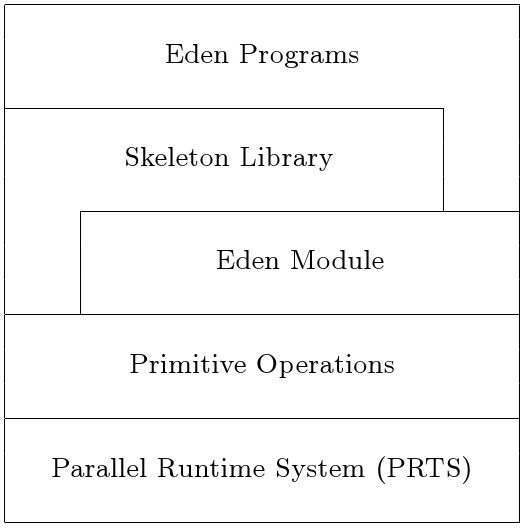
\includegraphics[width=5cm]{edenstructure.png}
\end{figure}

Supports PVM and MPI middleware.

We use EDI, the Eden Implementation Language, a type-safe wrapper
around the primitive operations.
\end{frame}

\begin{frame}
\frametitle{Conceptually}

A \textbf{channel} connects the outport of a thread with an inport of
a receiver thread.  The channel consists of a writing end and a
placeholder for reading.

\pause

A channel can be a \textbf{stream} (list), where elements are sent
one-by-one.

\pause

Each machine runs a process, consisting of multiple threads, with a
one-to-one relation between threads and outports.

\pause

Sending is explicit and asynchronous, receiving is implicit and
blocking.

\pause

When the reading placeholder is identified as garbage, the process
holding the writing end can be terminated.
\end{frame}

\begin{frame}[fragile]
\frametitle{Concretely}

\begin{verbatim}
data ChanName' a = Chan Int# Int# Int#
createC :: IO ( ChanName' a, a )
spawnProcessAt :: Int -> IO () -> IO ()
sendWith :: Strategy a -> ChanName' a -> a -> IO ()
\end{verbatim}
\pause
Low-level interface:
\begin{verbatim}
connectToPort :: ChanName' a -> IO ()
sendData :: Mode -> a -> IO ()
data Mode = Connect
           | Data
           | Stream
           | Instantiate Int
\end{verbatim}

\end{frame}

\begin{frame}
  \frametitle{Par Monad}
  Par can be used for specifying \textbf{pure parallel computations} in which the order of the computation is not known beforehand. \newline
  
  The programmer specifies how \textbf{information flows} from one part of the computation to another, but not the order in which computations will be evaluated at runtime. Information flow is described using variables called \texttt{IVars}, which support \texttt{put} and \texttt{get} operations. \newline 
  
  \tiny{\texttt{http://hackage.haskell.org/packages/archive/monad-par/0.1.0.1/doc/html/Control-Monad-Par.html}}
\end{frame}

\begin{frame}[fragile]
  \frametitle{Par Monad - Par}
  \begin{lstlisting}[language=Haskell]
fork :: Par () -> Par ()
runPar :: Par a -> a
  \end{lstlisting}
\end{frame}

\begin{frame}[fragile]
  \frametitle{Par Monad - Par}
  \begin{lstlisting}[language=Haskell]
fork :: Par () -> Par ()
  \end{lstlisting}

  Forks a computation to happen in parallel.
\end{frame}

\begin{frame}[fragile]
  \frametitle{Par Monad - Par}
  \begin{lstlisting}[language=Haskell]
runPar :: Par a -> a
  \end{lstlisting}

  Run the parallel computations and get the value.
\end{frame}

\begin{frame}[fragile]
  \frametitle{Par Monad - IVar}
  \begin{lstlisting}[language=Haskell]
new :: Par (IVar a)
get :: IVar a -> Par a
put :: NFData a => IVar a -> a -> Par ()
  \end{lstlisting}
\end{frame}

\begin{frame}[fragile]
  \frametitle{Par Monad - IVar}
  \begin{lstlisting}[language=Haskell]
get :: IVar a -> Par a  
  \end{lstlisting}

  Read the value in a IVar. The get can only return when the value 
  has been written by a prior or parallel put to the same IVar.
  
  % Reading the value doesn't remove it as takeMVar would
\end{frame}

\begin{frame}[fragile]
  \frametitle{Par Monad - IVar}
  \begin{lstlisting}[language=Haskell]
put :: NFData a => IVar a -> a -> Par ()
  \end{lstlisting} 
    
  Put a value into a IVar. \textbf{Multiple puts} to the same IVar \textbf{are not 
    allowed}, and result in a runtime error.
    
  % This is different than MVar as you can write that multiple times.
\end{frame}

\begin{frame}
  \frametitle{Par Monad - IVar vs. MVar}
  \begin{itemize}
    \item IVar: One-to-Many communication
    \item MVar: One-to-One communication
  \end{itemize}
\end{frame}

\begin{frame}[fragile]
  \frametitle{Par Monad - Example}
  \begin{lstlisting}[language=Haskell]
                      a
                     / \  
                    b   c
                     \ /
                      d
  
runPar $ do
       [a,b,c,d] <- sequence [new,new,new,new]
       fork $ do x <- get a; put b (x+1)
       fork $ do x <- get a; put c (x+2)
       fork $ do x <- get b
                 y <- get c 
                 put d (x+y)
       fork $ do put a (3 :: Int)
       get d
  \end{lstlisting}
\end{frame}


\begin{frame}
\frametitle{EDI backend for monad-par}
\end{frame}
\end{document}
